%%
%% Copyright (c) 2018 The Authors.  All Rights Reserved.
%%
%% Weitian LI, et al.
%% School of Physics and Astronomy, Shanghai Jiao Tong University,
%% Shanghai, China.
%%
%% 2018-08-23
%%

% Class options:
% - letters : for papers in the journal's Letters section (<=5 pages)
% - onecolumn : single column
% - doublespacing : double line spacing (do NOT submit in this format)
% - usenatbib : (always use this) use `natbib' package for citations
% - usegraphicx : includes the `graphicx' package
% - useAMS : support 3 upright Greek characters
% - usedcolumn : use `dcolumn' package for table column alignment

\documentclass[fleqn,usenatbib]{mnras}
\newlength{\myfigwidth}
\setlength{\myfigwidth}{\columnwidth}

%------ internal review ------
%\documentclass[fleqn,usenatbib,onecolumn]{mnras}
%\setlength{\myfigwidth}{0.5\columnwidth}
%\geometry{top=35mm,bottom=35mm,left=30mm,right=30mm}
%\linespread{1.5}

%\usepackage{xeCJK}
%\setCJKmainfont{Noto Serif CJK SC}
%\xeCJKsetup{PunctStyle=kaiming}
%------ internal review ------

\usepackage{newtxtext,newtxmath}
\usepackage[T1]{fontenc}
\usepackage{ae,aecompl}

%
% Custom packages
%
\usepackage{graphicx}
\usepackage{amsmath}
\usepackage{amssymb}
\usepackage{siunitx}  % typeset units; from `texlive-science'

% Workaround the error:
%   \pdfendlink ended up in different nesting level than \pdfstartlink
% Credit: https://tex.stackexchange.com/a/154184
\hypersetup{draft}

\graphicspath{{./}{figures/}}  % NOTE: the trailing '/' matters

\sisetup{
  range-phrase=\text{--},
  range-units=single,
  product-units=repeat,
  list-separator={, },
  list-final-separator={, and },
  separate-uncertainty=true,
}
\DeclareSIUnit\MHz{\mega\hertz}
\DeclareSIUnit\kHz{\kilo\hertz}
\DeclareSIUnit\jansky{Jy}
\DeclareSIUnit\mJy{\milli\jansky}
\DeclareSIUnit\mK{\milli\kelvin}
\DeclareSIUnit\parsec{pc}
\DeclareSIUnit\Mpc{\mega\parsec}

\def\sectionautorefname{Section}
\def\subsectionautorefname{Section}
\def\figureautorefname{Fig.}
\def\tableautorefname{Table}

%
% Custom commands
%
\newcommand{\R}[1]{\mathrm{#1}}
\newcommand{\B}[1]{\mathbfit{#1}}

% Help track changes
% Credit: https://tex.stackexchange.com/a/49913
\newcommand{\editdone}[1]{{#1}}
\newcommand{\editwip}[1]{{\leavevmode\color{magenta}#1}}
\newcommand{\editone}[1]{{\leavevmode\color{cyan}#1}}
\newcommand{\edittwo}[1]{{\leavevmode\color{magenta}#1}}


%%======================================================================
%% Title page
%%

%      ............................................. (<=45 chars)
\title[EoR Signal Separation with a CDAE]{%
  Separating the EoR Signal with a Convolutional Denoising Autoencoder:
  a Deep-learning-based Method
}

% If you need two or more lines of authors, add an extra line using \newauthor
\author[Li~et~al.]{%
Weitian Li,$^{1}$\thanks{E-mail:
  \href{mailto:liweitianux@sjtu.edu.cn}{liweitianux@sjtu.edu.cn} (WL);
  \href{mailto:hgxu@sjtu.edu.cn}{hgxu@sjtu.edu.cn} (HX)}
Haiguang Xu,$^{1,2}$\footnotemark[1]
Zhixian Ma,$^{3}$
Ruimin Zhu,$^{4}$
Dan Hu,$^{1}$
Zhenghao Zhu,$^{1}$
\newauthor  % start on a new line
Chenxi Shan,$^{1}$
Jie Zhu$^{3}$
and
Xiang-Ping Wu$^{5}$
\\
% List of institutions
$^{1}${School of Physics and Astronomy,
  Shanghai Jiao Tong University,
  800 Dongchuan Road, Shanghai 200240, China} \\
$^{2}${Tsung-Dao Lee Institute / IFSA Collaborative Innovation Center,
  Shanghai Jiao Tong University,
  800 Dongchuan Road, Shanghai 200240, China} \\
$^{3}${Department of Electronic Engineering,
  Shanghai Jiao Tong University,
  800 Dongchuan Road, Shanghai 200240, China} \\
$^{4}${Department of Statistics,
  Northwestern University,
  2006 Sheridan Road, Evanston, IL 60208, US} \\
$^{5}${National Astronomical Observatories,
  Chinese Academy of Sciences,
  20A Datun Road, Beijing 100012, China}
}

% These dates will be filled out by the publisher
\date{Accepted XXX. Received YYY; in original form ZZZ}

% Enter the current year, for the copyright statements etc.
\pubyear{2018}

% Don't change these lines
\begin{document}
\label{firstpage}
\pagerange{\pageref{firstpage}--\pageref{lastpage}}
\maketitle

%
% Abstract
% (<=200 words for Letters, <=250 words for Articles)
%
\begin{abstract}
When applying the foreground removal methods to uncover the
\editone{faint cosmological signal from the epoch of reionization (EoR)},
the foreground spectra are assumed to be smooth.
However, this assumption can be seriously violated in practice since
the unresolved or mis-subtracted foreground sources, which are further
complicated by the frequency-dependent beam effects of interferometers,
will generate significant fluctuations along the frequency dimension.
To address this issue, we propose a novel deep-learning-based method
that uses a 9-layer convolutional denoising autoencoder (CDAE) to
separate the EoR signal.
After being trained on the SKA images simulated with realistic beam
effects, the CDAE achieves excellent performance as the correlation
coefficient ($\rho$) between the reconstructed and input EoR signals
reaches \editwip{\num{0.929 +- 0.045}}.
In comparison, \editwip{the traditional polynomial fitting method and
continuous wavelet transform method both fail to uncover the EoR signal,
yielding $\rho_{\R{poly}} = \num{0.296 +- 0.121}$ and
$\rho_{\R{cwt}} = \num{0.1982+- 0.160}$, respectively.} % editwip
We conclude that, by hierarchically learning sophisticated features
through multiple convolutional layers, the CDAE is a powerful tool that
can be used to overcome the complicated frequency-dependent beam effects
and accurately separate the EoR signal, which exhibits the great
potential of deep-learning-based methods in future EoR experiments.
\end{abstract}

% Select between one and six entries from the list of approved keywords.
% Don't make up new ones.
% https://academic.oup.com/DocumentLibrary/mnras/keywords.pdf
\begin{keywords}
methods: data analysis --
techniques: interferometric --
dark ages, reionization, first stars --
radio continuum: general
\end{keywords}


%%======================================================================
%% Paper body
%%

\section{Introduction}
\label{sec:intro}

The \SI{21}{\cm} line emission of neutral hydrogen from the epoch of
reionization (EoR) is regarded as a decisive probe to directly explore
this stage (see \citealt{furlanetto2016rev} for a review).
To detect the \SI{21}{\cm} signal, which is believed to have been
redshifted to the frequencies below \SI{200}{\MHz}, low-frequency
radio interferometers such as the SKA \citep{koopmans2015rev} and its
pathfinders have been built or under construction.
The observational challenges, however, are immense due to
complicated instrumental effects, ionospheric distortions, radio frequency
interference, and the strong foreground contamination that
overwhelms the EoR signal by about \numrange{4}{5} orders of magnitude
(see \citealt{morales2010rev} for a review).
Fortunately, in the frequency dimension the foreground contamination
is expected to be intrinsically smooth, while the EoR signal fluctuates
rapidly on $\lesssim \si{\MHz}$ scales.
This difference is the key characteristic exploited by many
foreground removal methods in order to uncover the faint EoR signal
\citep[e.g.,][]{wang2006,liu2009fgrm,harker2009,wang2013,gu2013}.

However, the smoothness of the foreground spectra can be destroyed by
the frequency-dependent beam effects, i.e., the variation of the point
spread function (PSF) with frequencies that cannot be perfectly
calibrated \citep{liu2009ps}.
Because of the incomplete $uv$ coverage,
the PSF has a complicated profile consisting of a narrow peaky main lobe
and a multitude of jagged side lobes with relative amplitudes of about
\numrange{0.1}{1} per cent that extend beyond the field of view (FoV)
\citep[e.g.,][their figures 1 and 3]{liu2009ps}.
A source that is unresolved or mis-subtracted (e.g., due to the limited
FoV) during the CLEAN process leaves catastrophic residuals,
the locations of which vary with the frequency since the angular
position of a PSF side lobe is inversely proportional to the frequency.
These effects lead to complicated residuals fluctuating along the
frequency dimension, which cannot be correctly separated from the EoR
signal by the traditional foreground removal methods that rely on
the smoothness of the foreground spectra.

Given the complicated profiles and frequency-dependent variations of
the PSF, it would be difficult to craft a practicable model for most,
if not all, existing foreground removal methods to overcome the beam
effects, even at the cost of extensive computation burden
\citep[e.g.,][]{lochner2015}.
Therefore deep-learning-based methods, which can distil knowledge from
the data to automatically refine the model, seem more feasible
and appealing \citep[e.g.,][]{herbel2018,vafaeiSadr2018}.
In recent years, the deep learning algorithms have seen prosperous
developments and have brought breakthroughs into many fields
(see \citealt{lecun2015} for a recent review).
Among various deep learning algorithms, the convolutional denoising
autoencoder (CDAE) and its variants are flexible and powerful in
learning subtle and complicated features from the data and have been
successfully applied to
weak gravitational wave signal denoising \citep[e.g.,][]{shen2017},
monaural audio source separation \citep[e.g.,][]{grais2017}, and so on.
These applications have demonstrated the outstanding abilities of the
CDAE in extracting weak signals from highly temporal-variable data,
thus it is worth trying to apply the CDAE to separate the EoR signal.
Although the signal-to-noise ratio in the EoR detection is much lower
than in existing applications, the EoR signal and foreground emission
as well as the beam effects are stationary or semi-stationary.

In this paper, a novel deep-learning-based method that uses a CDAE
is proposed to tackle the complicated frequency-dependent beam effects
and to separate the EoR signal along the frequency dimension.
In \autoref{sec:method}, we introduce the CDAE and elaborate
the proposed method.
In \autoref{sec:experiments}, we demonstrate the performance of the
CDAE by applying it to the simulated SKA images
\editwip{and briefly explain how the CDAE learns}.
We discuss the method and carry out
\editwip{comparisons to traditional methods}
in \autoref{sec:discussions}.
Finally, we summarise our work in \autoref{sec:summary}.
The implementation code and data are made public at
\url{https://github.com/lwieitianux/cdae-eor}.


%%======================================================================
\section{Methodology}
\label{sec:method}

%%----------------------------------------------------------------------
\subsection{Convolutional denoising autoencoder}
\label{sec:cdae}

An autoencoder is composed of an encoder and a decoder, which can be
characterised by the functions $f(\cdot)$ and $g(\cdot)$, respectively.
The encoder maps the input $\B{x}$ to an internal code $\B{h}$, i.e.,
$\B{h} = f(\B{x})$, and the decoder tries to reconstruct the wanted
signal from the code $\B{h}$, i.e., $\B{r} = g(\B{h})$, where $\B{x}$,
$\B{h}$, and $\B{r}$ are all vectors for this work.
By placing constraints (e.g., dimensionality, sparsity) on the
internal code $\B{h}$ and training the autoencoder to minimize the
loss $L(\B{r}, \, \B{x})$, which quantifies the difference between the
reconstruction $\B{r}$ and the input $\B{x}$, the autoencoder tries to
learn the codes that effectively represent the input data
\citep[e.g.,][chapter 14]{goodfellow2016}.

\editwip{%
In order to make the autoencoder learn good representations of the input
data instead of simply copying the input as the output,
\citet{vincent2008,vincent2010} proposed to apply the denoising criterion,
which states that `a good representation is one that can be obtained
robustly from a corrupted input and that will be useful for recovering the
corresponding clear input.'
The input data are artificially corrupted (e.g., by adding noise) and the
autoencoder is trained to reconstruct the original clean input for the
purpose of learning robust features from the input data.
In addition, the trained autoencoder can be employed to denoise the data
\citep[e.g.,][]{xie2012,gondara2016}, hence being called a `denoising
autoencoder.'

Classic autoencoders use fully connected layers and thus have a large
number of parameters, which are harder to train and prevent from build
deeper and more powerful autoencoders
\citep[e.g.,][]{glorot2010,larochelle2009}.
On the other hand, convolutional layers as used in convolutional neural
networks (CNNs) have much fewer parameters and can better exploit the local
features in data.  Therefore it is easier and more intuitive to stack
multiple convolutional layers to build highly expressive CNNs that achieve
outstanding performance in image classification and relevant fields
\citep[e.g.,][]{krizhevsky2012,simonyan2014,szegedy2015}.
By utilising multiple convolutional layers instead of fully connected
layers in a denoising autoencoder, the resulting CDAE gains the similar
capabilities of CNNs to fully exploit the complicated features in the data
(e.g., the subtle differences between the EoR signal and foreground
emission when interlaced with the beam effects), which greatly improves
the denoising ability and can reconstruct even seriously corrupted signal
\citep{du2017}.}  % editwip
In consequence, the CDAE is well suited to separate the faint EoR signal
$\B{x}_{\R{eor}}$ from the strong foreground emission $\B{x}_{\R{fg}}$,
which is regarded as the noise, by denoising the input total emission
($\B{x} = \B{x}_{\R{eor}} + \B{x}_{\R{fg}}$).


%%----------------------------------------------------------------------
\subsection{Network architecture}
\label{sec:architecture}

\begin{figure*}
  \centering
  \includegraphics[width=0.9\textwidth]{network-crop}
  \caption{\label{fig:network}\editwip{%
    The network architecture of the proposed CDAE that consists of 9
    convolutional layers, which can be divided into the encoder (the orange
    boxes), the decoder (the blue boxes), and the output layer (the green
    bar).
    Each convolutional layer contains a number of filters (marked below the
    boxes) and an activation function (ELU for the encoder and decoder
    layers; `tanh' for the output layer).
    The batch normalisation (BN) is applied to all layers except for the
    first layer.
    Pooling and upsampling layers are not employed.
  }}
\end{figure*}

\editwip{%
The CDAE consists of multiple convolutional layers with each layer
containing a number of filters and an activation function.
Each filter is convolved with the output of the previous layer and the
convolution result then goes through the activation function to produce
the output of this layer.
Because the CDAE output $\B{r}$, which has the same size as the input
$\B{x}$, is a vector of length $n_f$ with $n_f$ being the number of
frequency channels in the image cube (see also \autoref{sec:simulation}),
the last convolutional layer (i.e., the output layer) has only one filter.
The remaining convolutional layers can be divided into the encoder and
decoder parts.
The number of layers in the encoder and decoder as well as the number of
filters in each layer are hyperparameters of the CDAE.

We adopt filters of size 3 in all layers, and use the hyperbolic tangent
function (i.e., tanh; see also \autoref{sec:preprocessing}) and the
exponential linear unit (ELU; \citealt{clevert2016}) as activation
functions for the output layer and other layers, respectively.
The batch normalisation is applied to all layers except for the first
layer, for which the input data are already normalised, to improve the
training process as well as to act as a regularizer to prevent overfitting
\citep{ioffe2015}.

We have followed common practices \citep[e.g.,][]{suganuma2018,geron2017}
to build multiple CDAE architectures, each containing a different number of
layers and filters.
After evaluating their performances (see also \autoref{sec:results}),} % editwip
the simplest one with sufficiently good performance is selected,
which consists of a 4-layer encoder with $(32,64,64,32)$ filters,
a 4-layer decoder with $(32,64,64,32)$ filters, and one output layer,
as illustrated in \autoref{fig:network}.
\editwip{%
We have also tested to use pairs of pooling and upsampling layers in the
CDAE, but it has very little impacts on the performance.
Moreover, we focus on the feature extraction and denoising abilities of the
CDAE rather than the specific formats of the internal codes.
Thus it is reasonable to not use pooling and upsampling layers, which also
eases the explanation of how the CDAE learns (\autoref{sec:explanation}).
}


%%----------------------------------------------------------------------
\subsection{Training and evaluation}
\label{sec:train-eval}

The CDAE is initialised by the He uniform initialiser \citep{he2015}
and is trained by using the Adam optimisation method \citep{kingma2015}.
The loss, which describes the difference between the reconstructed EoR
signal $\B{r}_{\R{eor}}$ and the input EoR signal $\B{x}_{\R{eor}}$,
is calculated as the mean squared error (MSE), i.e.,
\begin{equation}
  \label{eq:loss}
  L = \frac{1}{N} \sum_{i=1}^{N}
    \left[ \B{r}_{\R{eor}}^{(i)} - \B{x}_{\R{eor}}^{(i)} \right]^T
    \left[ \B{r}_{\R{eor}}^{(i)} - \B{x}_{\R{eor}}^{(i)} \right],
\end{equation}
where $N$ is the number of data points in the training dataset.
By being trained to minimize the loss $L$, the CDAE learns to
reconstruct the EoR signal from the input data $\B{x}$.

To evaluate the performance of the CDAE in separating the EoR signal,
the commonly used Pearson's correlation coefficient \editwip{(CC)}
\citep[e.g.,][]{harker2009,chapman2013}
is adopted to measure the similarity between the reconstructed EoR
signal $\B{r}_{\R{eor}}$ and the input EoR signal $\B{x}_{\R{eor}}$:
\begin{equation}
  \label{eq:corrcoef}
  \rho(\B{r}_{\R{eor}}, \B{x}_{\R{eor}})
      = \frac{\sum_{j=1}^{n}(r_{\R{eor},j} - \bar{r}_{\R{eor}})
      (x_{\R{eor},j} - \bar{x}_{\R{eor}})}{
        \sqrt{\sum_{j=1}^{n}(r_{\R{eor},j} - \bar{r}_{\R{eor}})^2
          \sum_{j=1}^{n}(x_{\R{eor},j} - \bar{x}_{\R{eor}})^2}
    },
\end{equation}
where $n$ is the length of the signals,
and $\bar{r}_{\R{eor}}$ and $\bar{x}_{\R{eor}}$ represent the mean values.
The closer the correlation coefficient is to one, the better the
performance of separation.


%%======================================================================
\section{Experiments}
\label{sec:experiments}

%%----------------------------------------------------------------------
\subsection{Simulation of the SKA images}
\label{sec:simulation}

We carry out end-to-end simulations to generate the SKA images to
train the proposed CDAE and evaluate its performance.
\editwip{%
An \SI{8}{\MHz} frequency band centred at \SI{158}{\MHz} is chosen as
an example and is divided into $n_f = 101$ channels with a resolution of
\SI{80}{\kHz}.
At each frequency, the sky maps of the foreground emission and the EoR
signal are simulated within an area of \SI{10 x 10}{\degree} and are
pixelized into \num{1800 x 1800} with a pixel size of \SI{20}{\arcsecond}.
For the foreground emission, we take into account the contributions from
the Galactic synchrotron and free-free radiations, extragalactic point
sources, and radio haloes.
The Galactic synchrotron radiation is simulated by extrapolating the Haslam
\SI{408}{\MHz} map with a power-law spectrum.  We make use of the
reprocessed Haslam \SI{408}{\MHz} map\footnote{%
  The reprocessed Haslam \SI{408}{\MHz} map:
  \url{http://www.jb.man.ac.uk/research/cosmos/haslam_map/}}
\citep{remazeilles2015} as the template, and the synchrotron spectral index
map made by \citet{giardino2002} to account for the index variation with
sky positions.
By employing the tight relation between the H$\alpha$ and free-free
emissions \citep[see][and references therein]{dickinson2003}, the Galactic
free-free radiation can be derived from the H$\alpha$ survey map
\citep{finkbeiner2003}.
Since the Galactic diffuse emissions vary remarkably across the sky, we
simulate them at a central position of (R.A., Dec\@.) = (\SI{0}{\degree},
\SI{-27}{\degree}), which has a high galactic latitude
($b = \SI{-78.5}{\degree}$) and thus is expected to be appropriate for
EoR observations.
We account for the following 5 types of extragalactic point sources:
(1) star-forming and starburst galaxies, (2) radio-quiet active galactic
nuclei (AGNs), (3) Fanaroff-Riley type I and type II AGNs, (4) GHz-peaked
spectrum AGNs, and (5) compact steep spectrum AGNs.
The former three types of sources are simulated by utilizing the results
published by \citet{wilman2008} and the latter two types are simulated by
employing their corresponding luminosity functions and spectral models.
Similar to the real-time peeling of the brightest point sources in
practical data analysis pipelines \citep[e.g.,][]{mitchell2008,intema2009},
we assume that sources with a \SI{158}{\MHz} flux density
$S_{158} > \SI{10}{\mJy}$ have been removed \citep[e.g.,][]{liu2009ps}.
The radio haloes are simulated by generating a sample of galaxy clusters
with the Press-Schechter formalism \citep{press1974} and then applying
multiple scaling relations (e.g., between cluster mass and X-ray
temperature, between X-ray temperature and radio power) to derive their
radio emissions.
More details regarding to the simulation of these foreground components can
be found in our previous work \citep{wang2010} and references therein.
For simulating the sky maps of the EoR signal, we take advantage of the
2016 data release from the Evolution Of 21\,cm Structure project\footnote{%
  The Evolution Of 21\,cm Structure project:
  \url{http://homepage.sns.it/mesinger/EOS.html}}
\citep{mesinger2016} and extract the image slices at needed redshifts
(i.e., frequencies) from the light-cone cubes of the recommended `faint
galaxies' case.

\begin{figure*}
  \centering
  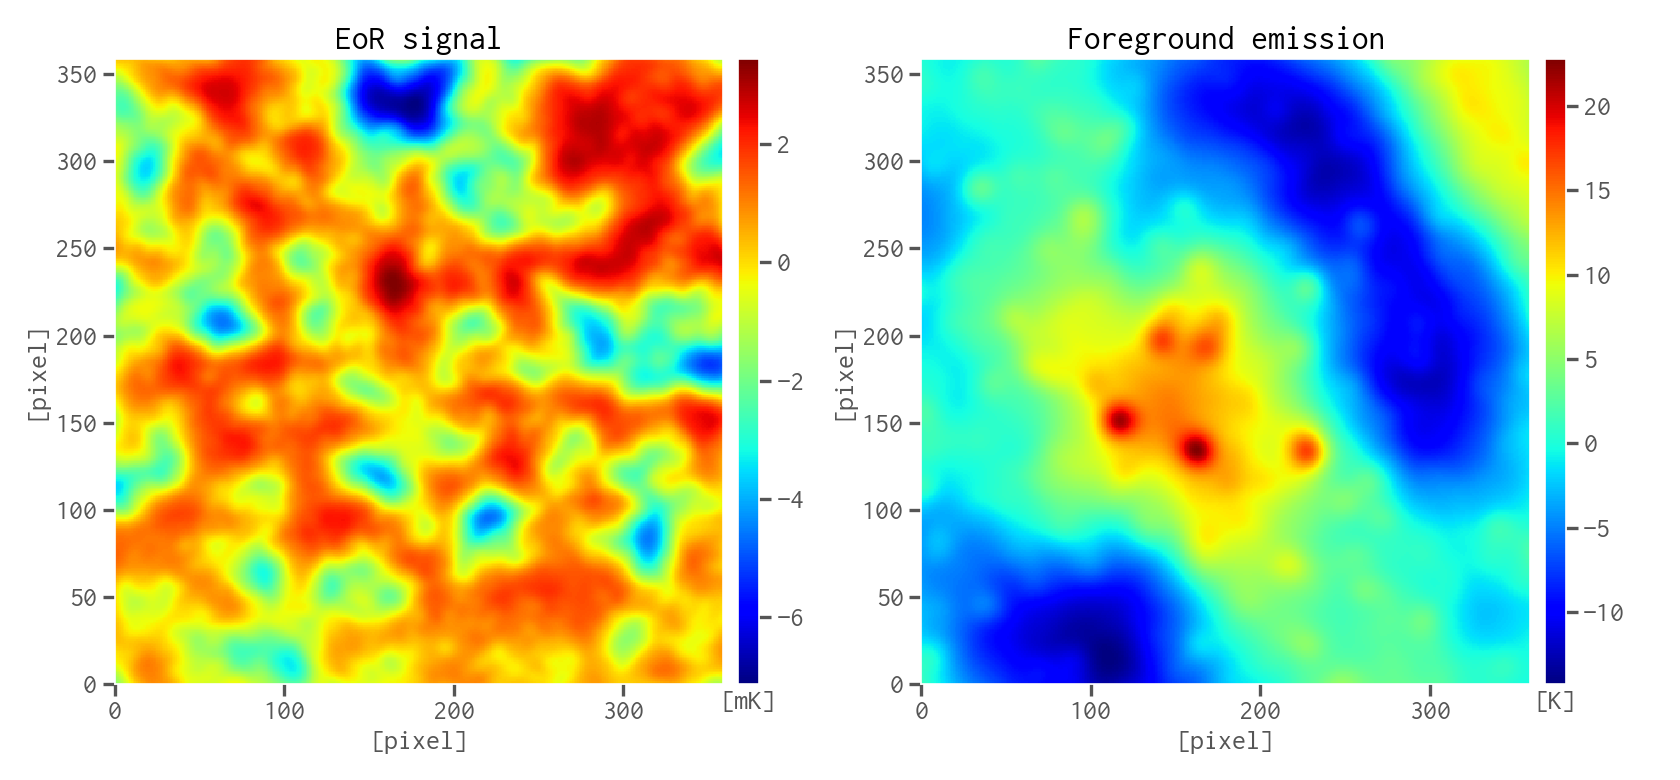
\includegraphics[width=0.8\textwidth]{obsimg-158}
  \caption{\label{fig:obsimg}\editwip{%
    Simulated images of the EoR signal (left panel) and the foreground
    emission (right panel) at \SI{158}{\MHz}.
    Both images have a size of \num{360 x 360} and cover a sky area of
    \SI{2 x 2}{\degree}.
    The blobs in the right panel show the bright point sources and radio
    haloes.
  }}
\end{figure*}

To fully incorporate realistic frequency-dependent beam effects into the
simulated sky images, we further adopt the SKA1-Low layout
configuration\footnote{\raggedright%
  SKA1-Low layout:
  \url{https://astronomers.skatelescope.org/wp-content/uploads/2016/09/SKA-TEL-SKO-0000422_02_SKA1_LowConfigurationCoordinates-1.pdf}}
to simulate instrument observations.
For each sky image, we employ the SKA1-Low layout in the
\textsc{oskar}\footnote{%
  OSKAR: \url{https://github.com/OxfordSKA/OSKAR} (version 2.7.0)}
simulator \citep{mort2010} to perform \SI{6}{\hour} synthesis imaging,
yielding the visibility data, from which the `observed'
image is created by the \textsc{wsclean}\footnote{%
  WSClean: \url{https://sourceforge.net/p/wsclean} (version 2.5)}
imager \citep{offringa2014}.
In order to emphasize the faint and relatively diffuse EoR signal, the
natural weighting and only baselines of \numrange{30}{1000} wavelengths are
utilized in the imaging process.} % editwip
Finally, the created images are cropped to keep only the central
\SI{2 x 2}{\degree} regions (i.e., \num{360 x 360} pixels) for the
purpose of the best quality.
Therefore, we obtain \editwip{a pair of} image cubes of size
\num{360 x 360 x 101} for the EoR signal $\left( C_{\R{eor}}^{(1)} \right)$
and the foreground emission $\left( C_{\R{fg}}^{(1)} \right)$, respectively
\editwip{%
(see \autoref{fig:obsimg} for the simulated images at \SI{158}{\MHz}).
To better illustrate the impacts of beam effects on the foreground spectra,
we show in \autoref{fig:simudata} the root-mean-square (r.m.s\@.) spectra
and the corresponding differential spectra of the foreground image cubes
with and without the beam effects considered.
Compared to the ideal sky foreground (the top panel), the spectral
smoothness of the `observed' foreground is seriously damaged by the
significant fluctuations resulted from the beam effects (the bottom panel).
} % editwip

\begin{figure}
  \centering
  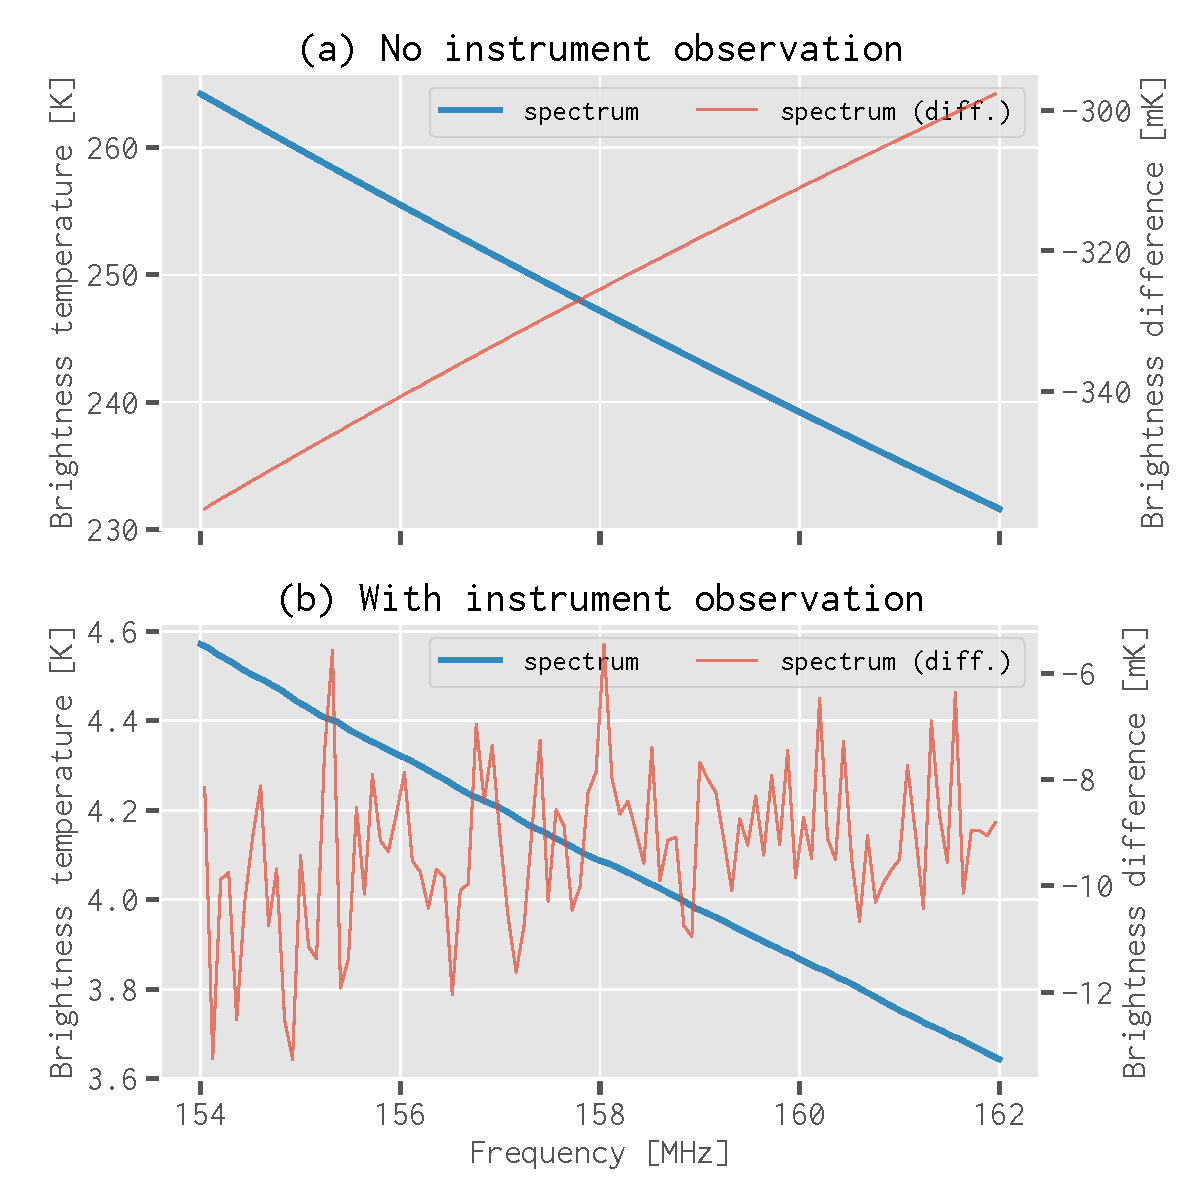
\includegraphics[width=\myfigwidth]{simudata}
  \caption{\label{fig:simudata}\editwip{%
    The r.m.s\@. spectra (the bold blue lines) and the corresponding
    differential spectra (the thin red lines) of the foreground image
    cubes.} % editwip
    The top and bottom panels show the cases without and with instrument
    observation, respectively.
  }
\end{figure}

\editwip{%
It is beneficial to simulate two pairs of image cubes, because we could use
one complete pair of them to evaluate the CDAE and hence illustrate its
performance more intuitively by presenting images and power spectra of the
separated EoR signal (see \autoref{sec:results}).
To obtain another pair of image cubes, we simulate the Galactic diffuse
emissions at a central coordinate of (R.A., Dec\@.) = (\SI{3}{\degree},
\SI{-27}{\degree}), i.e., \SI{3}{\degree} from the above pair of image
cubes, which is sufficient because the images are only \SI{2 x 2}{\degree}
in size.
Since extragalactic point sources, radio haloes, and the EoR signal are
mostly isotropic, we shift their sky maps simulated above by
\SI{3}{\degree} to generate the new sky maps.
Following the same procedures to simulate instrument observations, we
obtain the second pair of image cubes
$\left( C_{\R{eor}}^{(2)}, C_{\R{fg}}^{(2)} \right)$.

We note that the simulations do not include thermal noise because the
proposed method is currently designed to create tomographic EoR images
from very deep observations that have sufficiently low noise.
For example, SKA1-Low is expected to perform EoR imaging observations of
\SI{1000}{\hour} per pointing, reaching an unprecedented image noise level
of $\,\lesssim \SI{1}{\mK}$ \citep[e.g.,][]{mellema2013rev,koopmans2015rev}.
} % editwip


%%----------------------------------------------------------------------
\subsection{Data preprocessing}
\label{sec:preprocessing}

The dataset $S = \{(\B{x}, \,\B{x}_{\R{eor}})\}$ for the CDAE is derived
from the simulated image cubes $C_{\R{eor}}$ and $C_{\R{fg}}$, each data
point $(\B{x} = \B{x}_{\R{eor}} + \B{x}_{\R{fg}}, \,\B{x}_{\R{eor}})$
representing the total emission and the EoR signal of one sky pixel,
respectively.
\editwip{%
The dataset thus has $N_S = \num{360x360 x 2} = \num{259200}$
data points in total.}

For the input data $X = \{\B{x}\}$, we propose to apply the
Fourier Transform (FT) along the frequency dimension,
which makes the EoR signal more distinguishable from the
foreground emission and thus easier to be learned by the CDAE
(a comparison with the results derived without applying the FT is
presented in \autoref{sec:why-ft}).
The Blackman-Nuttall window function is applied to suppress the
FT side-lobes caused by the sharp discontinuities at both ends
of the finite frequency band \citep[e.g.,][]{chapman2016}.
It is sufficient to keep only half the Fourier coefficients because
$\B{x}$ is real, thus $\B{x}$ of length $n_f = 101$ is transformed to
be 51 complex Fourier coefficients, among which the $n_{\R{ex}}$
coefficients of the lowest Fourier frequencies are excised since they
are mostly contributed by the spectral-smooth foreground emission.
We adopt $n_{\R{ex}} = 6$ to achieve a balance between the foreground
suppression and the loss of the EoR signal.
The real and imaginary parts of the remaining 45 complex coefficients
are then concatenated into a new real vector of length $n_d = 90$,
since the CDAE requires real data.
Finally, the data are zero-centred and normalised to have unit variance.

The preprocessing steps for the input EoR signal
$X_{\R{eor}} = \{\B{x}_{\R{eor}}\}$
are basically the same except for minor adjustments.
After applying the FT, excising the $n_{\R{ex}}$ lowest Fourier
components, and concatenating the real and imaginary parts,
the data elements that have a value less than the 1$^{\R{st}}$
percentile or greater than the 99$^{\R{th}}$ percentile are truncated,
in order to prevent the possible outliers hindering the training of
the CDAE.
Finally, the value range of the data is scaled to be $[-1, 1]$ by
dividing by the maximum absolute value,
which allows to use the `tanh' activation function whose value range
is also $[-1, 1]$ in the output layer of the CDAE
(\autoref{sec:architecture}).


%%----------------------------------------------------------------------
\subsection{Training and results}
\label{sec:results}

\editwip{%
The preprocessed data of the first cube pair
$\left( C_{\R{eor}}^{(1)}, C_{\R{fg}}^{(1)} \right)$
is randomly partitioned into:
(1) training set ($S_{\R{tr}}$; 80 per cent; \num{103680} data points)
to fit the weights of filters by minimizing the loss $L$;
(2) validation set ($S_{\R{val}}$; 20 per cent; \num{25920} data points)
to determine the hyperparameters (e.g., the number of layers and filters,
the choice of loss function).
The preprocessed data of the second cube pair
$\left( C_{\R{eor}}^{(2)}, C_{\R{fg}}^{(2)} \right)$
is used as the test set ($S_{\R{test}}$; \num{129600} data points) to
evaluate the performance of the trained CDAE.} % editwip

We implement the proposed CDAE using the
\textsc{Keras}\footnote{Keras: \url{https://keras.io}
  (\editwip{version 2.2.4})}
framework \citep{keras} with the
\textsc{TensorFlow}\footnote{TensorFlow:
  \url{https://www.tensorflow.org} (\editwip{version 1.12.0})}
back end \citep{tensorflow},
\editwip{%
which is accelerated by the \textsc{cuda}\footnote{\raggedright%
  CUDA: \url{https://developer.nvidia.com/cuda-zone} (version 9.1.85)}
toolkit.
The ELU has a negative saturation of $a = 1.0$ \citep{clevert2016}.
The Adam optimisation method uses the default values for the exponential
decay rates of the first moment estimates $\beta_1 = 0.9$ and of the
second moment estimates $\beta_2 = 0.999$ \citep{kingma2015}.
We adopt a small initial learning rate ($\alpha = \num{e-5}$) and train the
CDAE on the training set ($S_{\R{tr}}$) with a batch size of 100 until the
training loss converges, which takes 50 epochs.
} % editwip

\begin{figure}
  \centering
  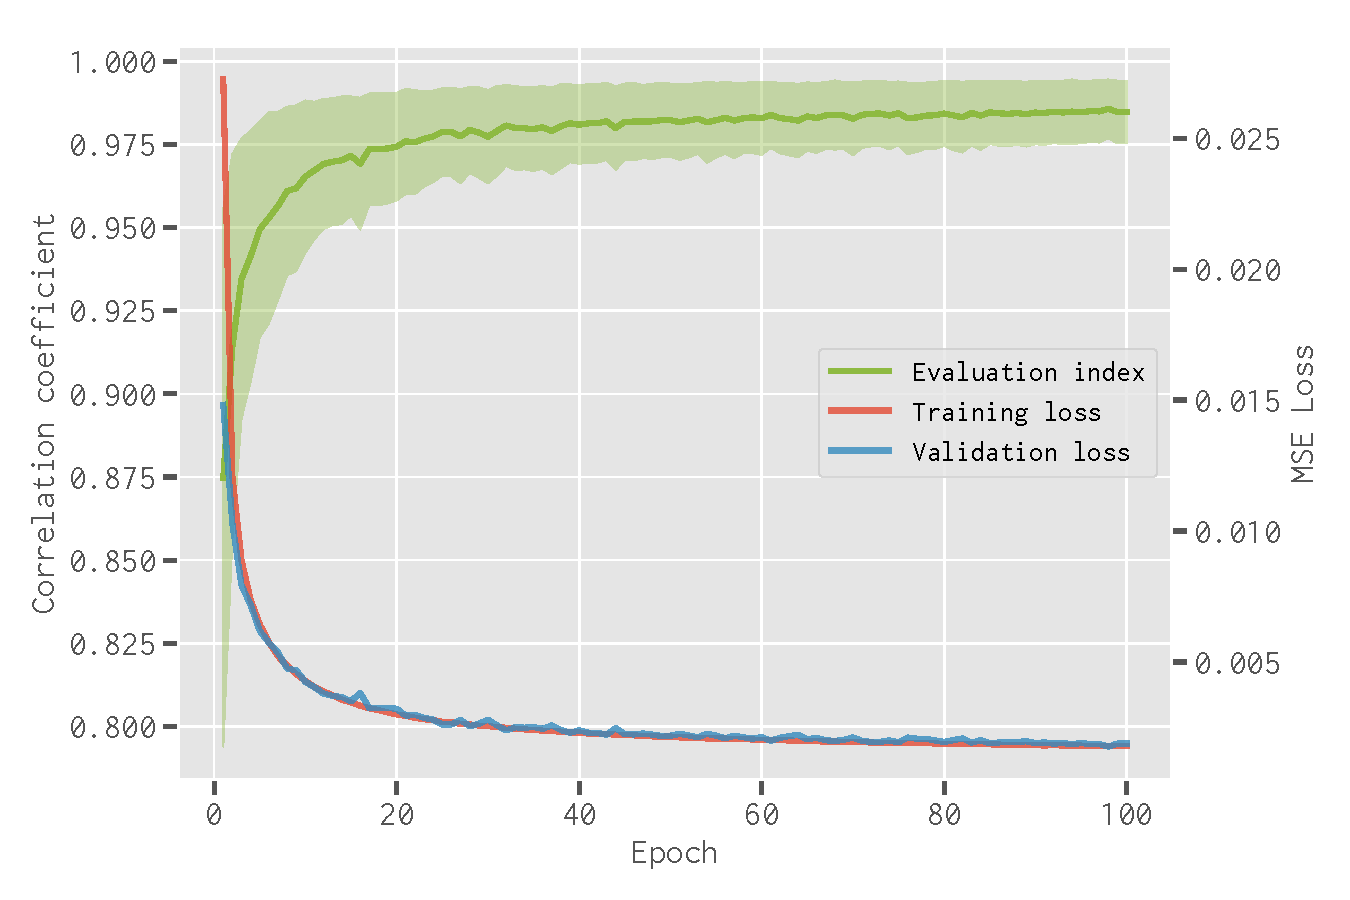
\includegraphics[width=\myfigwidth]{cdae-train}
  \caption{\label{fig:train}%
    The training loss (the solid red line), validation loss (the solid blue
    line), and correlation coefficient ($\rho$) calculated on the
    validation set $S_{\R{val}}$ (the \editwip{dashed blue} line with the
    shaded region representing the standard deviation) along the training
    of the CDAE.
  }
\end{figure}

\begin{figure}
  \centering
  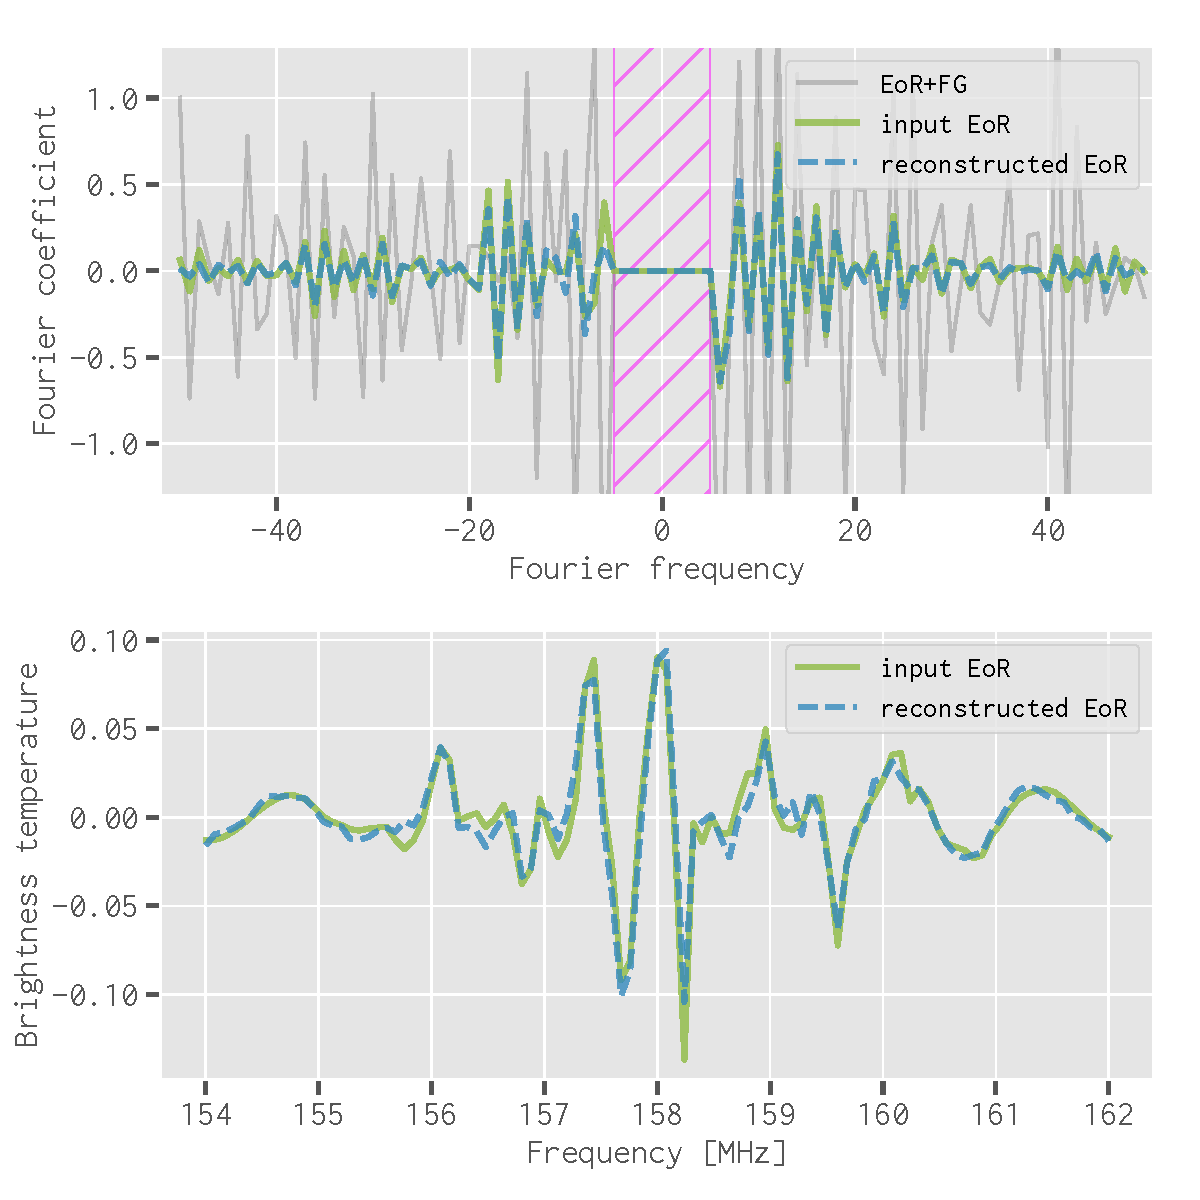
\includegraphics[width=\myfigwidth]{eor-result}
  \caption{\label{fig:eor-pix}%
    An example of the EoR signal reconstructed by the trained CDAE for
    one random pixel \editwip{in $S_{\R{test}}$}.
    \textbf{(top)} The input EoR signal $\B{x}_{\R{eor}}$ (the solid
    green line) and the reconstructed EoR signal $\B{r}_{\R{eor}}$
    (the dashed blue line) in the Fourier domain.
    \editwip{The correlation coefficient between the input and
      reconstructed EoR signals is $\rho = 0.931$.}
    The grey line represents the input total emission
    $\B{x} = \B{x}_{\R{fg}} + \B{x}_{\R{eor}}$.
    The magenta hatched region marks the excised Fourier coefficients
    in data preprocessing.
    \textbf{(bottom)} The input EoR signal $\B{x}_{\R{eor}}$ (the solid
    green line) and the reconstructed EoR signal $\B{r}_{\R{eor}}$
    (the dashed blue line) transformed back to the observing frequency
    domain.
  }
\end{figure}

The training and validation losses together with the evaluation index
(i.e., the correlation coefficient $\rho$) calculated on the validation set
$S_{\R{val}}$ during the training phase are shown in \autoref{fig:train}.
The steadily decreasing losses and increasing correlation coefficient
suggest that the CDAE is well trained without overfitting.
\editwip{%
After training, the correlation coefficient reaches
$\rho_{\R{val}} = \num{0.954 +- 0.029}$ on the validation set
$S_{\R{val}}$ and $\rho_{\R{test}} = \num{0.929 +- 0.045}$ on the test set
$S_{\R{test}}$, respectively.
This indicates that the trained CDAE can precisely reconstruct the EoR
signal and has excellent generalisation capability, which further confirms
that the CDAE has been well trained.} % ediwip
As an example, \autoref{fig:eor-pix} illustrates the reconstructed EoR
signal (\editwip{$\rho = 0.931$}) for one random pixel
\editwip{in $S_{\R{test}}$}.

\begin{figure*}
  \centering
  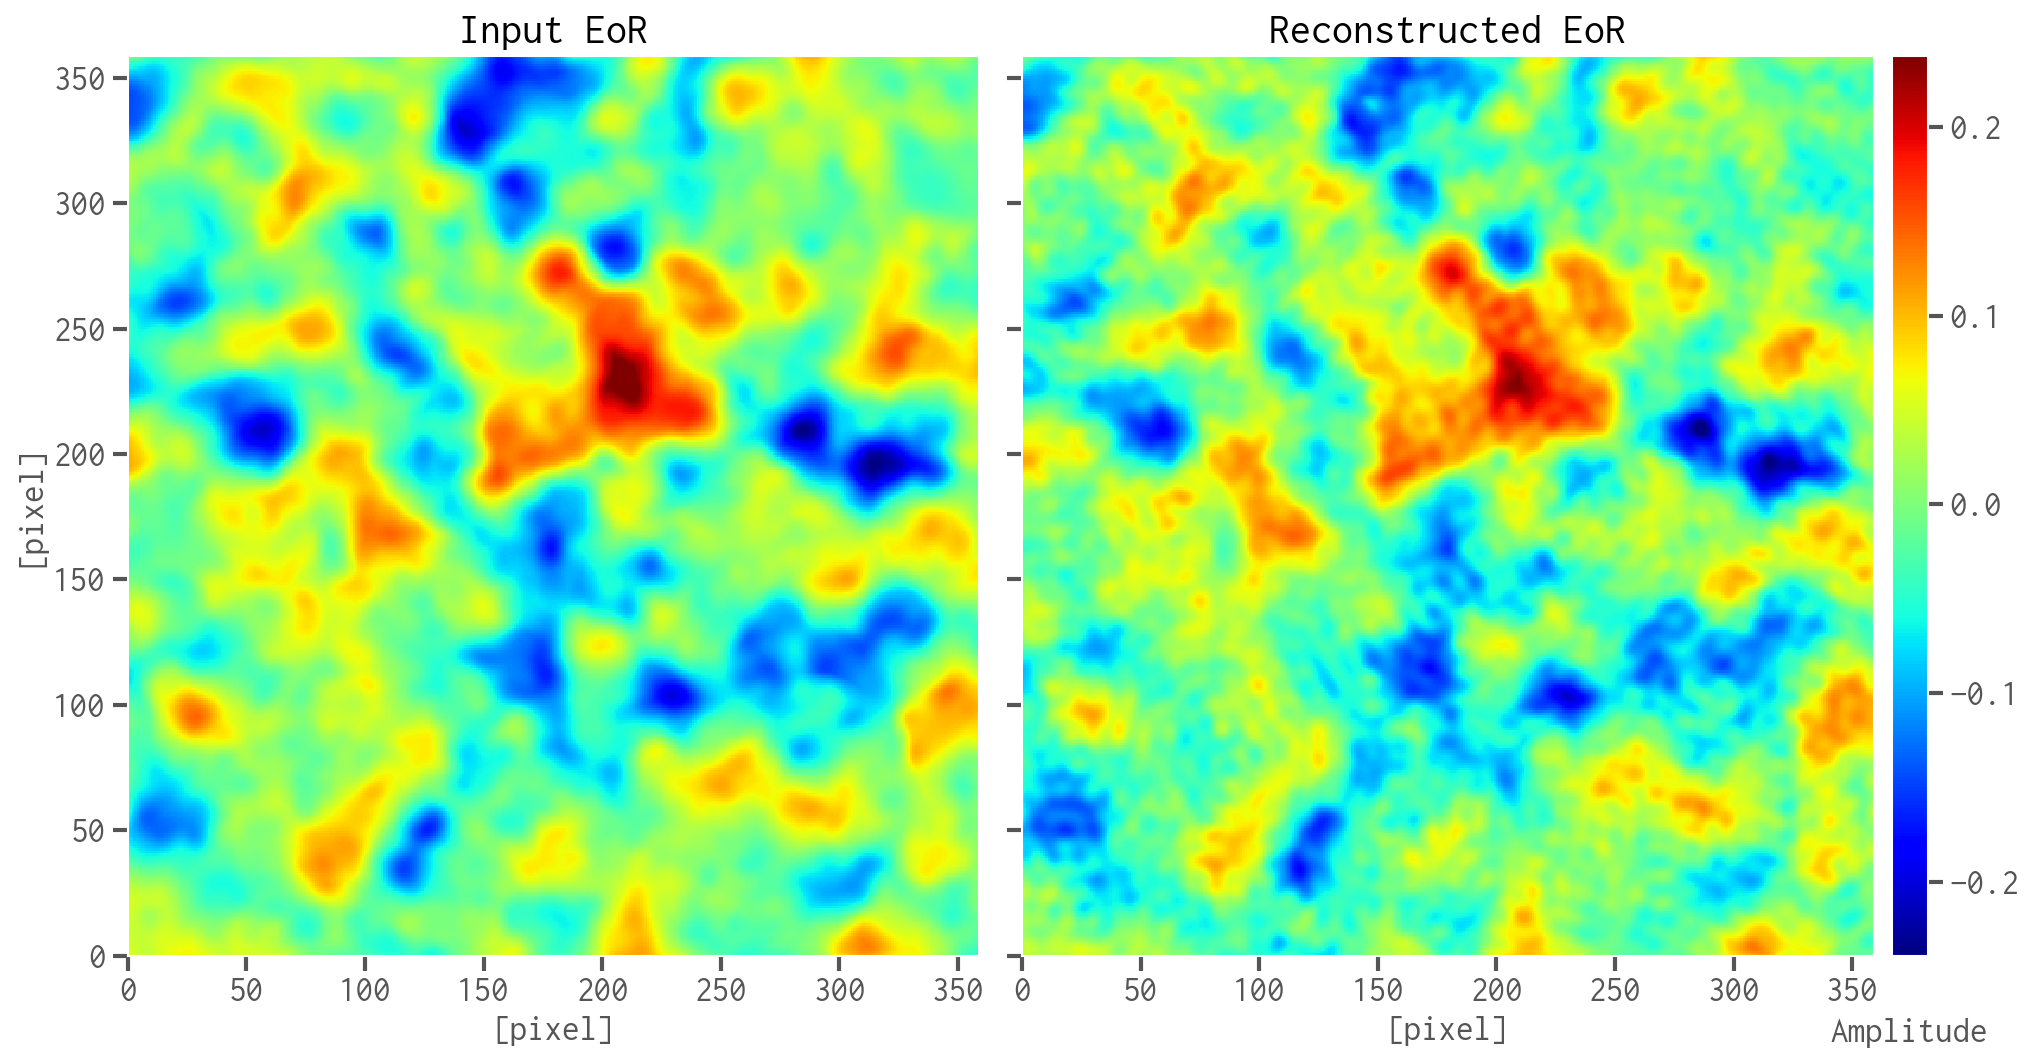
\includegraphics[width=0.8\textwidth]{eor-img-comp}
  \caption{\label{fig:eor-img}\editwip{%
    Comparison between the input EoR image (the left panel) and
    reconstructed EoR image (the right panel) at \SI{158}{\MHz}.
    The images have the same size (\num{360 x 360} pixel) and the figures
    share the same colour bar (the amplitude is normalised for the CDAE).
  }}
\end{figure*}

\begin{figure*}
  \centering
  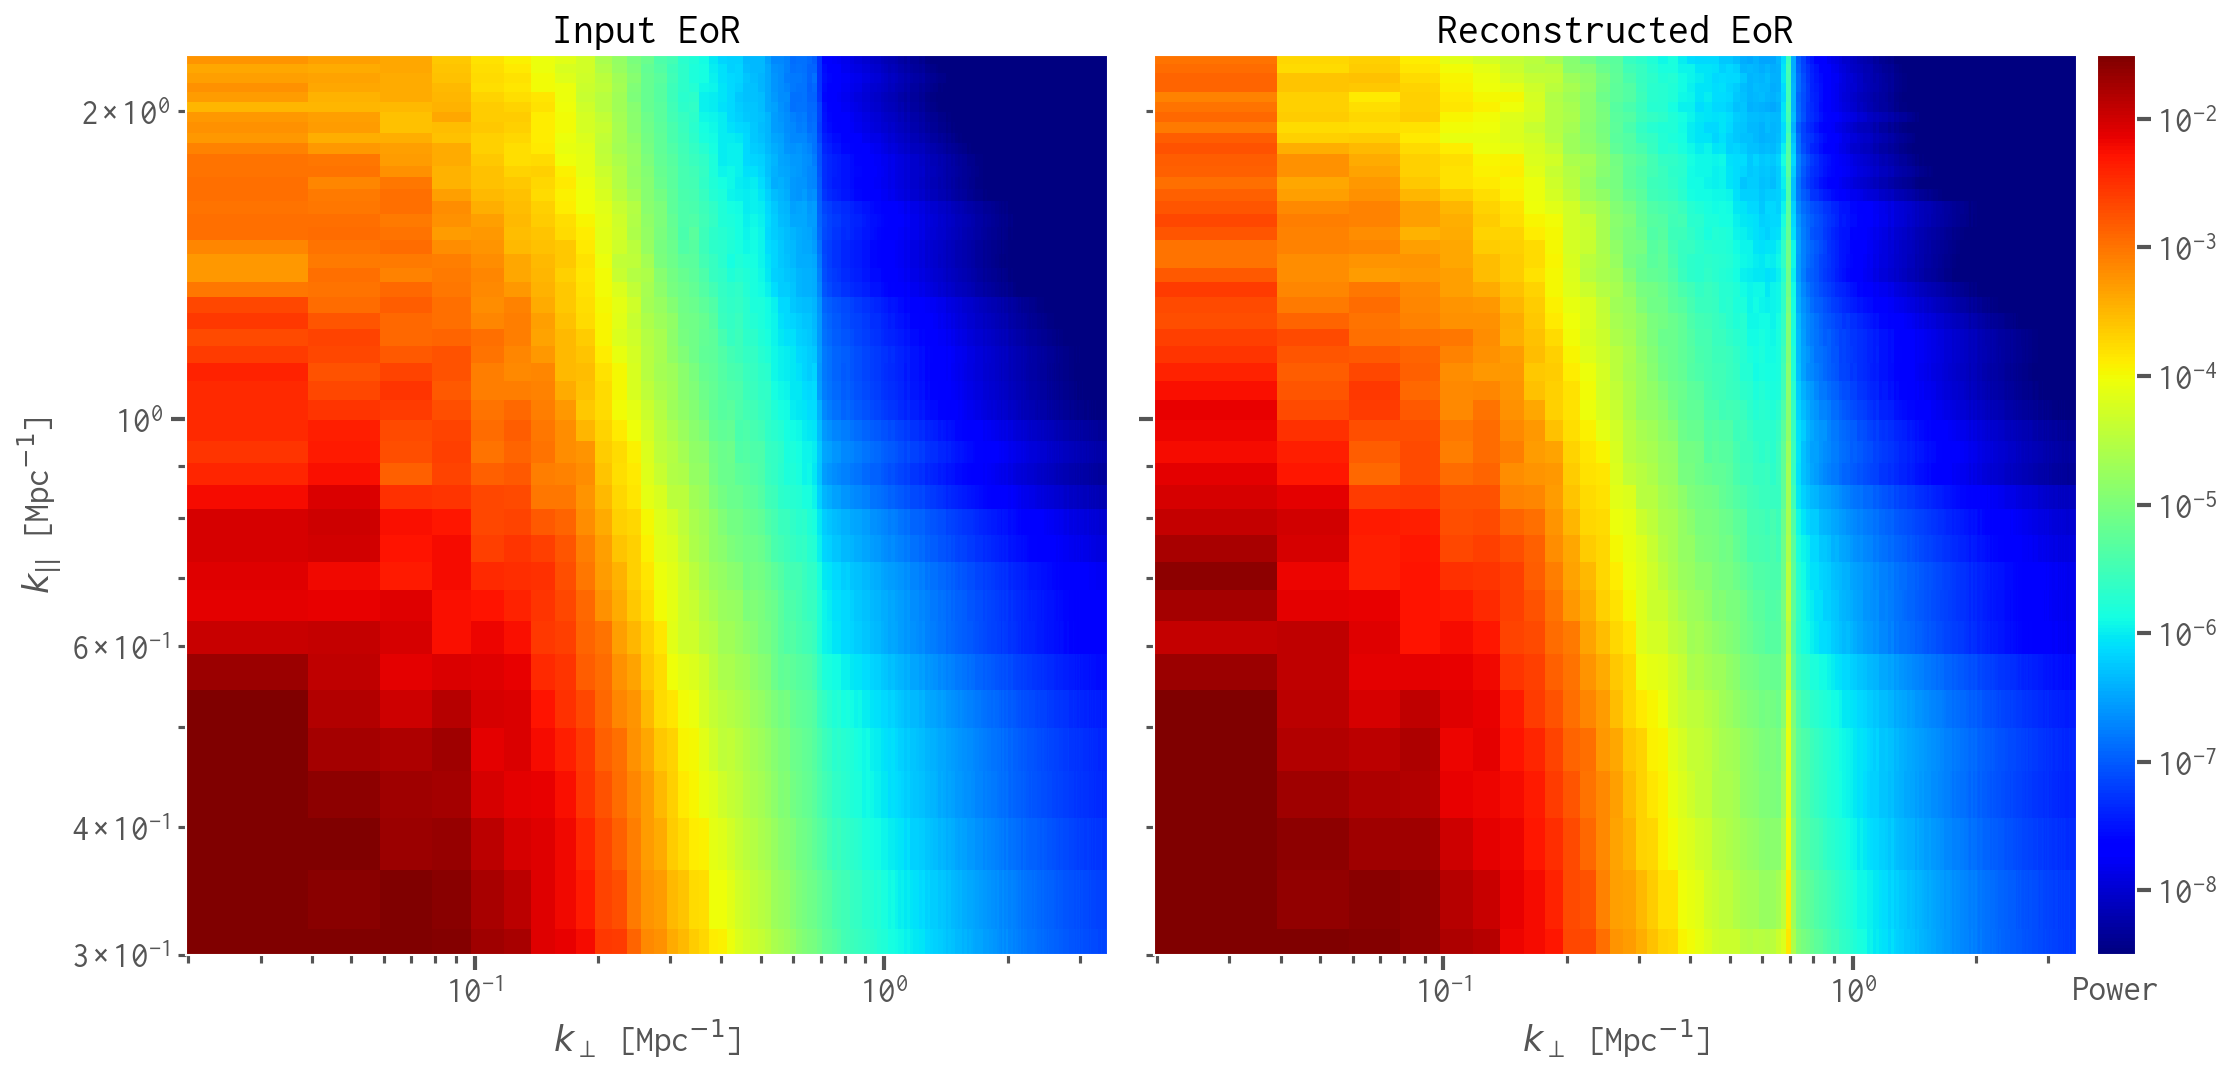
\includegraphics[width=0.8\textwidth]{eor-ps-comp}
  \caption{\label{fig:eor-ps}\editwip{%
    Comparison of 2D power spectra between the input (the left panel) and
    reconstructed (the right panel) EoR signals.
  }}
\end{figure*}

\editwip{%
Since the test set $S_{\R{test}}$ is derived from one complete pair of
simulated image cubes $\left( C_{\R{eor}}^{(2)}, C_{\R{fg}}^{(2)} \right)$,
we can make images of the reconstructed EoR signal and further calculate
the power spectrum.
As shown in \autoref{fig:eor-img} the images at \SI{158}{\MHz}, the
reconstructed EoR signal (the right panel) has almost identical structures
and amplitudes as the input EoR signal (the left panel).
We note that the reconstructed EoR image has small slight ripples, which
are associated with the excision of the $n_{\R{ex}}$ lowest Fourier
frequencies in data preprocessing (\autoref{sec:preprocessing}).
In addition, we calculate the two-dimensional (2D) power spectra from the
image cubes of the input and reconstructed EoR signals
(\autoref{fig:eor-ps}).
It illustrates that the trained CDAE successfully recovers the EoR signal
on all covered scales except for a very thin stripe region at
$k_{\bot} \approx \SI{0.7}{\per\Mpc}$, where extra powers are generated
by the aforementioned ripples in the reconstructed EoR images.
} % editwip

The achieved excellent performance of the CDAE can be mainly attributed
to the architecture of stacking multiple convolutional layers, which
implements a powerful feature extraction technique by hierarchically
combining the basic features learned in each layer to build more and
more sophisticated features \citep{lecun2015}.
Combined with the flexibility provided by the \num{53569} trainable
weights, the CDAE, after being well trained, can intelligently learn a
model that is optimised to accurately separate the faint EoR signal
\citep[e.g.,][]{domingos2012}.


%%----------------------------------------------------------------------
\editwip{%
\subsection{How does the CDAE learn?}
\label{sec:explanation}

\begin{figure*}
  \centering
  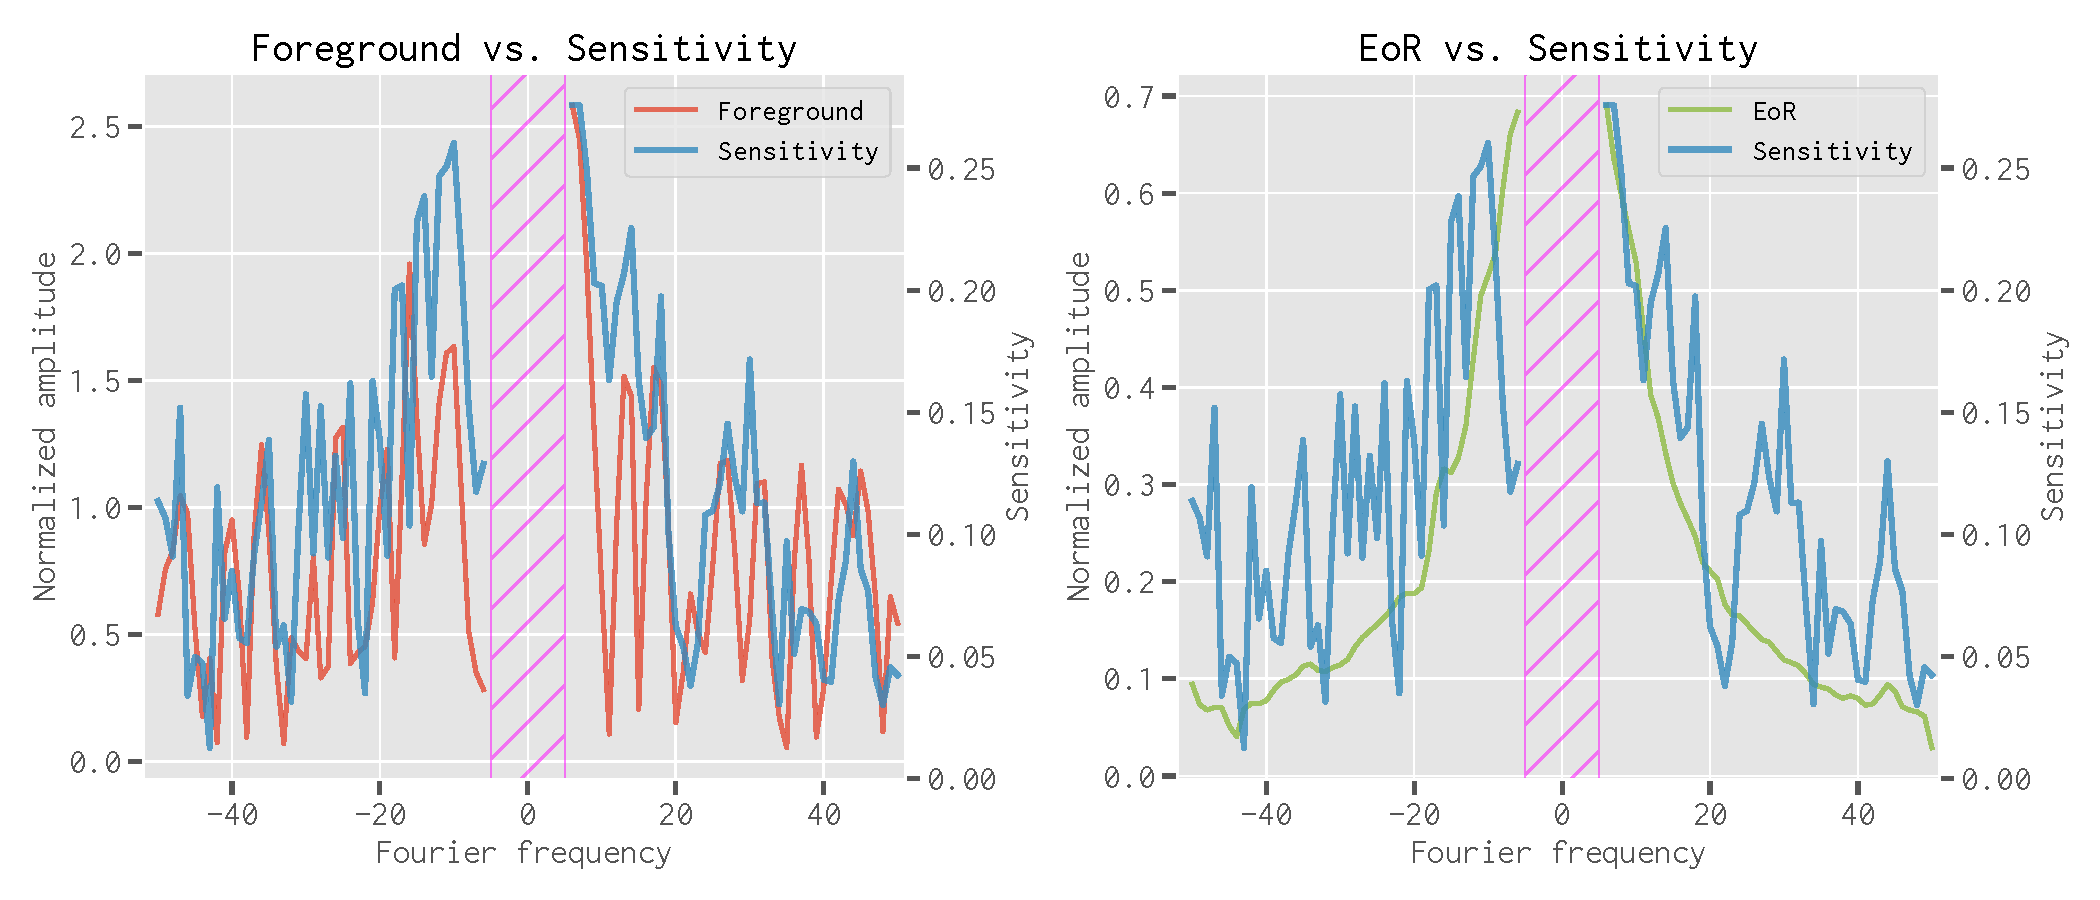
\includegraphics[width=0.8\textwidth]{occlusion-fgeor}
  \caption{\label{fig:occ-fgeor}\editwip{%
    The sensitivity distribution $\B{s}$ (the blue lines in both panels)
    obtained by applying the occlusion method.
    We also plot the r.m.s\@. amplitudes of the foreground emission
    ($\B{y}_{\R{fg}}$, the red line in the left panel) and the EoR signal
    ($\B{y}_{\R{eor}}$, the green line in the right panel).
    The sensitivity distribution is more correlated with the EoR signal
    [$\rho(\B{s}, \B{y}_{\R{eor}}) = 0.742$] than the foreground
    [$\rho(\B{s}, \B{y}_{\R{fg}}) = 0.562$].
  }}
\end{figure*}

\begin{figure}
  \centering
  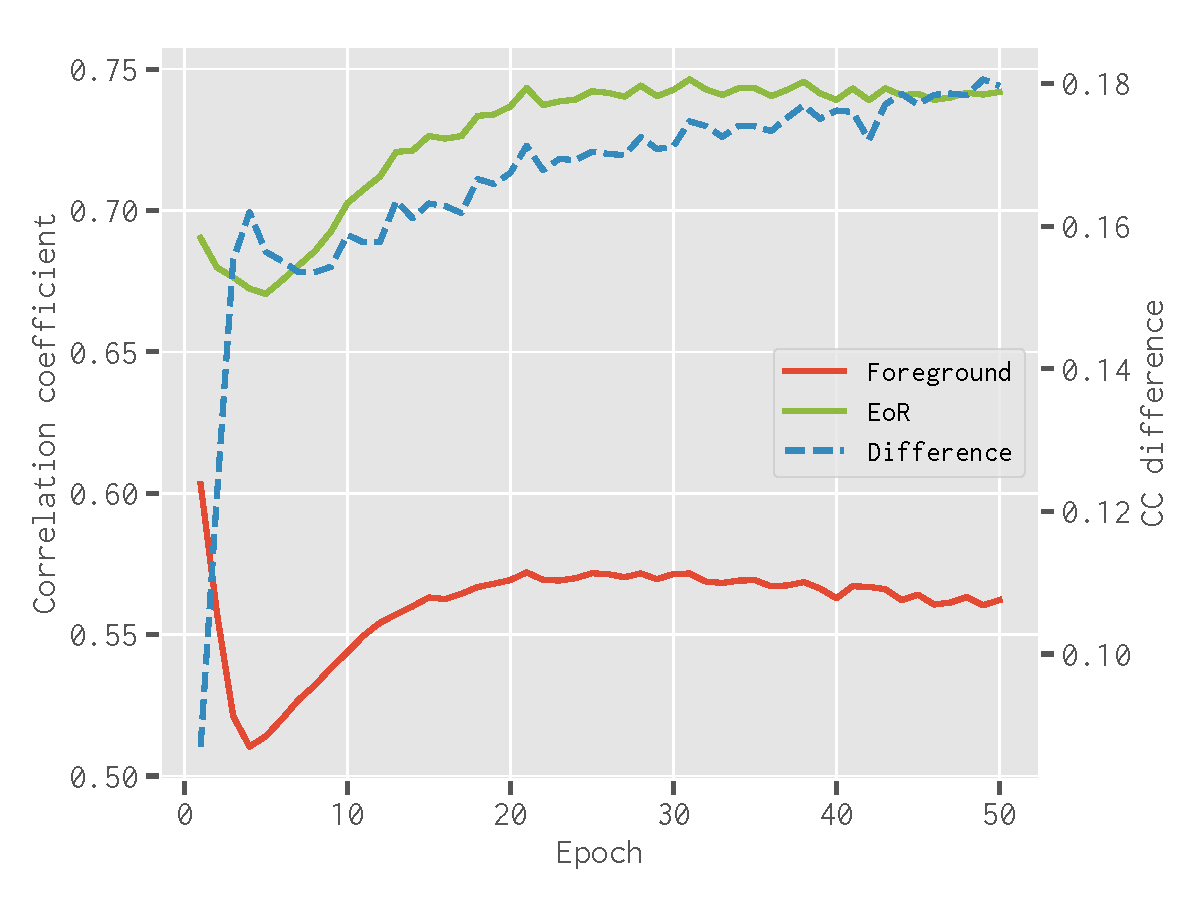
\includegraphics[width=\myfigwidth]{occlusion-epoch}
  \caption{\label{fig:occ-epoch}\editwip{%
    The variations of $\rho(\B{s}, \B{y}_{\R{fg}})$ (the solid red line),
    $\rho(\B{s}, \B{y}_{\R{eor}})$ (the solid green line), and their difference
    $d = \rho(\B{s}, \B{y}_{\R{eor}}) - \rho(\B{s}, \B{y}_{\R{fg}})$
    (the dashed blue line) along the training process.
  }}
\end{figure}

There is a growing sense that neural networks need to be interpretable to
humans.
However, the visualisation and interpretability of neural networks are
still outstanding challenges and are the frontier of deep learning studies
\citep[see][for recent reviews]{olah2017,olah2018}.
Over the years, the deep learning community has developed multiple methods
to help interpret neural networks
\citep[e.g.,][]{simonyan2013,zeiler2014,mahendran2015,springenberg2015}.
Considering that the proposed CDAE holds its own specificities, such as
that it learns to separate weak signal instead of performing
classifications and that the input data are are vectors rather than images,
most of the developed feature visualisation and interpretation methods
become inapplicable.
Therefore, we employ the occlusion method \citep{zeiler2014} to gain some
insights into how the CDAE learns to separate the EoR signal.

The occlusion method applies a mask to occlude a small portion of the input
data (e.g., an image) and then measure the induced performance loss.
By sliding the mask among the input data and recording the performance
loss, the sensitivities of each part of the data on the performance are
derived.
Then we can examine whether the signals or objects of interest have higher
sensitivities and thus determine whether the neural network actually learns
the right features from the data \citep{zeiler2014}.

To visualise the trained CDAE, we make use of the validation set
$S_{\R{val}}$ and apply a mask of length 3 to the input total emission
$\B{x}$, i.e., occluding 3 adjacent elements of the input vectors, and then
measure the sensitivity of the occluded part, which is calculated as the
occlusion-induced performance loss, i.e.,
\begin{equation}
  \label{eq:perf-loss}
  s = \rho(\B{r}_{\R{eor}}, \B{x}_{\R{eor}}) -
      \rho(\B{r}^*_{\R{eor}}, \B{x}_{\R{eor}}),
\end{equation}
where $\B{x}_{\R{eor}}$ is the input EoR signal, and
$\B{r}_{\R{eor}}$ and $\B{r}^*_{\R{eor}}$ are the reconstructed EoR signals
without and with occlusion, respectively.
By sliding the mask by one element and repeating the above calculation each
time, we obtain the sensitivity distribution $\B{s}$ at each Fourier
frequency, as shown in \autoref{fig:occ-fgeor}, where the r.m.s\@.
amplitudes of the foreground emission ($\B{y}_{\R{fg}}$) and the EoR signal
($\B{y}_{\R{fg}}$) are also plotted.
We find that the sensitivity distribution is more correlated with the EoR
signal [$\rho(\B{s}, \B{y}_{\R{eor}}) = 0.742$] than the foreground
[$\rho(\B{s}, \B{y}_{\R{fg}}) = 0.562$].
This verifies that the trained CDAE has learned to distinguish the EoR
signal from the foreground contamination and hence becomes more sensitive
to the data parts of higher signal-to-noise ratio.

In addition, to further interpret the learning process of the CDAE, we
apply the occlusion method at each epoch and derive the correlation
coefficients between the sensitivity distribution ($\B{s}$) and the
foreground emission ($\B{y}_{\R{fg}}$) and the EoR signal
($\B{y}_{\R{eor}}$), i.e., $\rho(\B{s}, \B{y}_{\R{fg}})$ and
$\rho(\B{s}, \B{y}_{\R{eor}})$, respectively.
In \autoref{fig:occ-epoch}, we present the variations of
$\rho(\B{s}, \B{y}_{\R{fg}})$, $\rho(\B{s}, \B{y}_{\R{eor}})$, and their
difference $d = \rho(\B{s}, \B{y}_{\R{eor}}) - \rho(\B{s}, \B{y}_{\R{fg}})$
along the training process.
During the first several epochs, the $\rho(\B{s}, \B{y}_{\R{fg}})$ drops
rapidly while the difference $d$ increases quickly, indicating the CDAE is
capturing the major structures of the EoR signal.
The small dip at about \numrange{4}{8} epochs for the difference $d$ may be
caused by the momentum method employed in the Adam optimisation algorithm
\citep{kingma2015}.
As the traning continues, the difference $d$ keeps increasing slowly, which
suggests that the CDAE is learning the fine characteristics of the EoR
signal to better distinguish it from the foreground emission.

None the less, how to rigorously interpret the CDAE remains an open
question.
Further works are essential to fully understand the CDAE in order to craft
more tailored and efficient neural networks for practical EoR signal
separation and various other applications.
} % editwip


%%======================================================================
\section{Discussions}
\label{sec:discussions}

%%----------------------------------------------------------------------
\subsection{Why preprocess the dataset with Fourier Transform?}
\label{sec:why-ft}

We have performed another experiment using the same CDAE architecture,
datasets, and data preprocessing steps, except for applying the FT
as depicted in \autoref{sec:preprocessing}.
After training the CDAE in the same way as described in
\autoref{sec:results}, \editwip{the correlation coefficients on the
validation set $S_{\R{test}}$ and test set $S_{\R{test}}$ reach only
$\rho_{\R{noft,val}} = \num{0.693 +- 0.137}$ and
$\rho_{\R{noft,test}} = \num{0.628 +- 0.167}$, respectively,
which indicates a worse performance compared to the case with FT applied.
As presented in \autoref{fig:train-noft}, the training loss decreases more
slowly and converges after about 100 epochs.} % editwip
We also find that the training process is slightly unstable given the small
spikes on the curves of both the loss and correlation coefficient.
These indicate that it is beneficial to preprocess the
dataset by applying the FT along the frequency dimension, because the
EoR signal and the foreground emission become more distinguishable
in the Fourier domain, where the fluctuating EoR signal concentrates on
larger Fourier modes while the spectral-smooth foreground emission
distributes mainly on smaller Fourier modes \citep[e.g.,][]{parsons2012}.

\begin{figure}
  \centering
  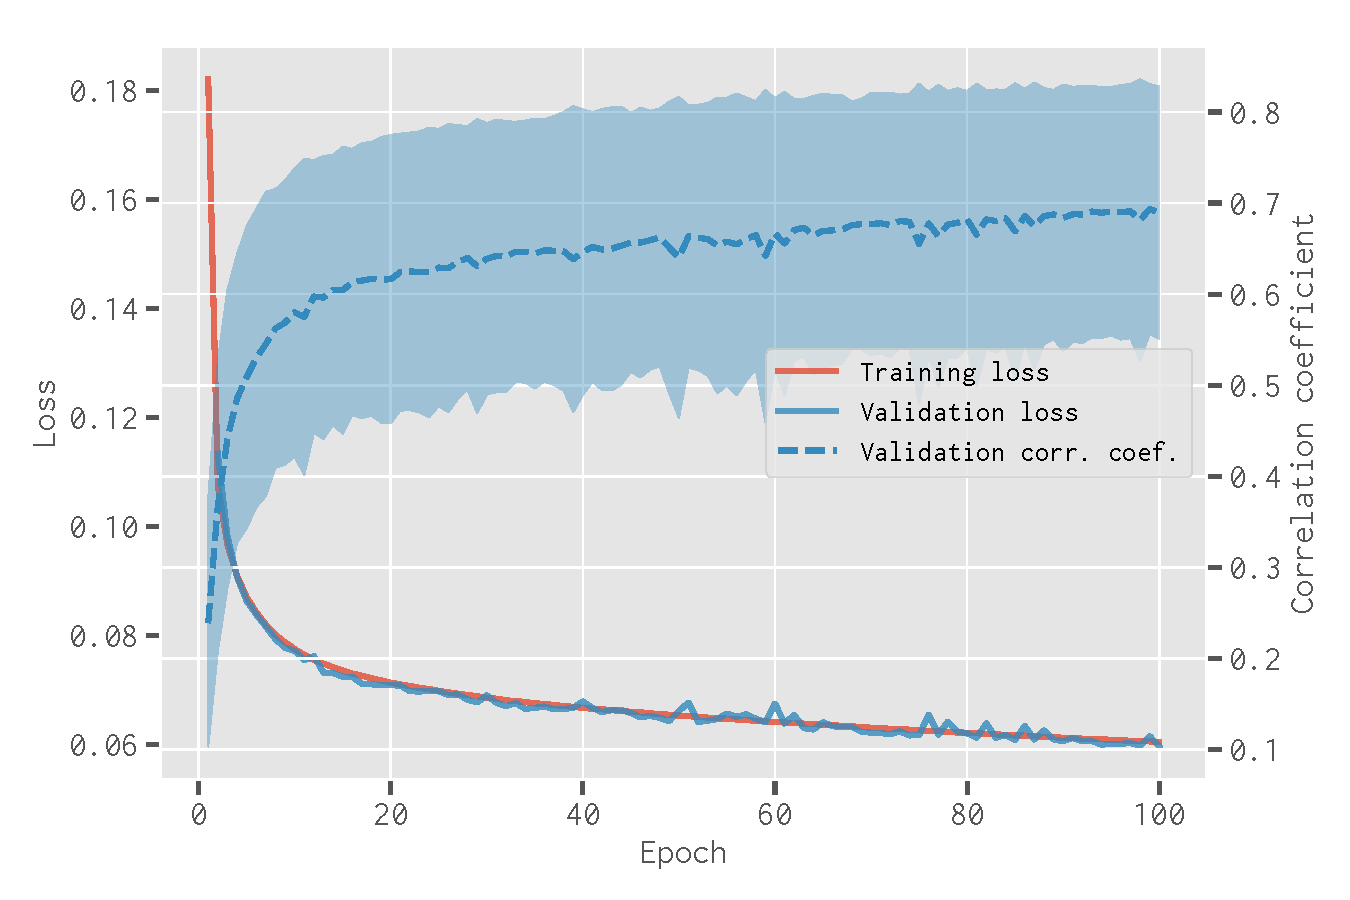
\includegraphics[width=\myfigwidth]{cdae-train-noft}
  \caption{\label{fig:train-noft}%
    Same as \autoref{fig:train} but for the case that the data are
    preprocessed without applying the FT.
  }
\end{figure}


%%----------------------------------------------------------------------
\editwip{%
\subsection{Comparing to traditional methods}
\label{sec:comparisons}

A variety of methods have been proposed to remove the foreground
contamination with the aim of revealing the faint EoR signal.
These methods can be broadly classified into two categories:
(1) parametric methods that apply a parametric model (e.g., a low-degree
polynomial) to fit and remove the foreground emission
\citep[e.g.,][]{wang2006,liu2009fgrm,wang2013};
(2) non-parametric methods, which do not assume a specific parametric model
for the foreground emission but exploit the differences between the
foreground emission and the EoR signal (e.g., their different spectral
features) to separate them
\citep[e.g.,][]{harker2009,gu2013,chapman2013,mertens2018}.

In order to further demonstrate the performance of our method, we compare
it to the polynomial fitting method \citep[e.g.,][]{wang2006} and the
continuous wavelet transform (CWT) method \citep{gu2013}.
Among the traditional methods, these two methods are chosen due to
following reasons:
(1) they both perform foreground removal along the frequency dimension
pixel-by-pixel, the same operation scheme as our method;
(2) they are one of the typical parametric and non-parametric methods,
respectively;
(3) they can give consistent and reliable results since they are intuitive
to implement and use.

With the polynomial fitting method,} % editwip
a low-degree polynomial is fitted along the frequency dimension for each
sky pixel in the image cube of the total emission (i.e.,
$C_{\R{tot}} = C_{\R{eor}} + C_{\R{fg}}$).
Then by subtracting the fitted smooth component, which is regarded as
the foreground emission, the EoR signal is expected to be uncovered.
\editwip{Using the same image cubes
\editwip{$\left( C_{\R{eor}}^{(2)}, C_{\R{fg}}^{(2)} \right)$}
simulated in \autoref{sec:simulation},} % editwip
we have tested polynomials of the degree from 2 (quadratic) to
5 (quintic), and find that the quartic polynomial (degree of 4)
can give the best result.
However, the correlation coefficient calculated for the separated EoR
signal in such a case is only
\editwip{$\rho_{\R{poly}} = \num{0.296 +- 0.121}$},
which indicates that the polynomial fitting method performs poorly in
removing the foreground emission.

\editwip{%
The CWT method works based on the assumption that the foreground emission
is spectrally smooth while the EoR signal spectral fluctuates rapidly.
Since their characteristic scales are significantly different, after
applying the CWT, the foreground emission can be easily distinguished from
the EoR signal in the wavelet coefficient space and thus be removed
\citep{gu2013}.
For each sky pixel, the CWT with the Morlet mother wavelet function is
applied to transform the spectrum to the wavelet coefficient space, where
the coefficients contributed by the foreground emission are filtered out by
utilising an appropriate mask.
The remaining coefficients are then inversely transformed to derive the
spectrum with foreground removed.
By evaluating on the same dataset
$\left( C_{\R{eor}}^{(2)}, C_{\R{fg}}^{(2)} \right)$,
we have tuned the method parameters (minimum scale $s_{\R{min}}$, maximum
scale $s_{\R{max}}$, number of scales $n_s$, and cone of influence $c_i$)
and adopt $s_{\R{min}} = 7.4$, $s_{\R{max}} = 50.0$, $n_s = 50$, and
$c_i = 1.6$ to obtain the relatively best performance, which, however, is
only $\rho_{\R{cwt}} = \num{0.1982+- 0.160}$.

The main reason that both traditional foreground removal methods can only
obtain remarkably inferior results is that the smoothness of the foreground
spectra is seriously damaged by the frequency-dependent beam effects, which
cause significant fluctuations of strength the same order as the EoR signal
on the originally smooth foreground spectra [\autoref{fig:simudata}(b)].
Therefore, the foreground spectra complicated by the beam effects cannot be
well modelled by a low-degree polynomial and have more similar
characteristic scales as the EoR signal.
As a result, both methods are unable to well model the complicated
foreground spectra and thus fail to remove them accurately.} % editwip
On the contrary, given its flexibility and data-driven nature,
the CDAE can distil knowledge from the data to optimise itself for
the EoR signal separation and hence achieve superior performance.


%%======================================================================
\section{Summary}
\label{sec:summary}

The frequency-dependent beam effects of interferometers can cause
rapid fluctuations along the frequency dimension,
which destroy the smoothness of the foreground spectra and prevent
traditional foreground removal methods from uncovering the EoR signal.
Given the difficulties in crafting practicable models to overcome the
complicated beam effects, methods that can intelligently learn tailored
models from the data seem more feasible and appealing.
To this end, we have proposed a deep-learning-based method that uses
a 9-layer CDAE to separate the EoR signal.
The CDAE has been trained on the simulated SKA images and has achieved
excellent performance.
We conclude that the CDAE has outstanding ability to overcome the
complicated beam effects and accurately separate the faint EoR signal,
exhibiting the great potential of deep-learning-based methods
to play an important role in the forthcoming EoR experiments.


%%======================================================================
\section*{Acknowledgements}

We thank the anonymous reviewer for the useful comments that helped
improve the manuscript.
We also thank Jeffrey Hsu for reading the manuscript and providing
helpful suggestions.
This work is supported by
the Ministry of Science and Technology of China
(grant Nos. 2018YFA0404601, 2017YFF0210903),
and the National Natural Science Foundation of China
(grant Nos. 11433002, 11621303, 11835009, 61371147).


%%======================================================================
%% References

\bibliographystyle{mnras}
\bibliography{references}


%%======================================================================
%% Appendix

% \appendix


%%======================================================================
% Don't change these lines
\bsp	% typesetting comment
\label{lastpage}
\end{document}

%% EOF
